\section{Protocol and results}
\label{sec:results}

\paragraph{Protocol.}
One checkpoint, one configuration, all 97 configurations; nothing tuned
or selected on GIFT-Eval data. The harness restates the official
protocol next to its sources (measured convention drift: zero on MASE,
$\sim$2.7\% on CRPS); aggregates are geometric-mean ratios vs seasonal
naive. Checkpoints are selected by intermediate evaluation, a doctrine
forced by measurement: validation loss designated the wrong checkpoint
three times out of three, once with a perfectly clean curve. The single
test-time augmentation is the sign flip,
$\hat{q}_\tau(x) = \tfrac{1}{2}[q_\tau(x) - q_{1-\tau}(-x)]$, the one
symmetry Lemma~\ref{lem:affine} leaves; precedents include TimesFM,
YingLong, and the 0.15M TinyCast
\citep{das2024timesfm,yinglong2025}. Table~\ref{tab:tta} shows why it
is alone. We refuse multi-checkpoint ensembling, and report every aggregate
plain and with flip.

\begin{table}[t]
\centering
\scriptsize
\begin{tabular}{llll}
\toprule
Variant & MASE & CRPS & Verdict \\
\midrule
none (champion, plain) & 0.895 & 0.624 & reference \\
sign flip & \textbf{0.870} & \textbf{0.596} & official ($2\times$ cost) \\
scale $f(kx)/k$ & = & = & identity (Lemma~\ref{lem:affine}) \\
time shift (origins $-1..{-7}$) & 0.898 & 0.627 & staleness beats phase \\
multi-lookback & 0.896 & 0.623 & worse with flip \\
context 2048 at inference & 1.190 & 0.876 & must be trained \\
\bottomrule
\end{tabular}
\caption{Test-time variants: under a normalization that quotients the
affine group, the sign is the only symmetry left.}
\label{tab:tta}
\end{table}

\begin{figure*}[t]
\centering
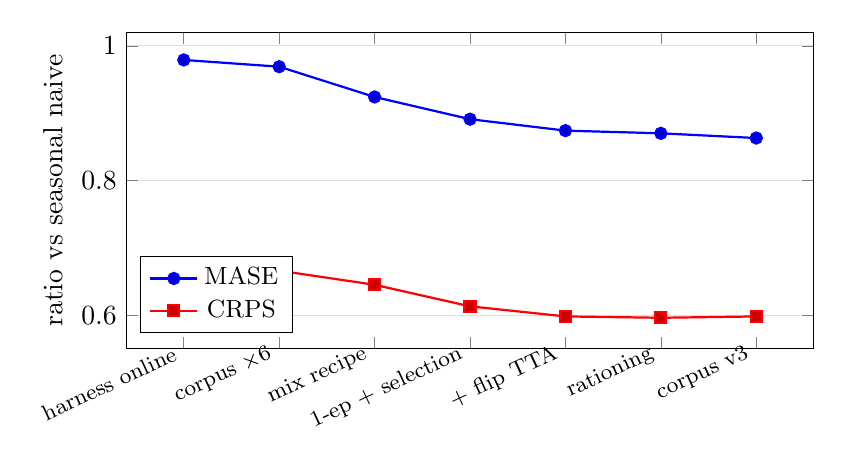
\begin{tikzpicture}
\begin{axis}[
  width=0.85\textwidth, height=5.6cm,
  ymin=0.55, ymax=1.02,
  ylabel={ratio vs seasonal naive},
  symbolic x coords={harness online, corpus $\times$6, mix recipe, 1-ep + selection, + flip TTA, rationing, corpus v3},
  xtick=data, x tick label style={rotate=25, anchor=east, font=\footnotesize},
  ymajorgrids, grid style={gray!25},
  legend style={font=\small, at={(0.02,0.05)}, anchor=south west},
  every axis plot/.append style={thick, mark=*}]
\addplot coordinates {(harness online,0.979) (corpus $\times$6,0.969)
  (mix recipe,0.924) (1-ep + selection,0.891) (+ flip TTA,0.874)
  (rationing,0.870) (corpus v3,0.863)};
\addplot coordinates {(harness online,0.677) (corpus $\times$6,0.666)
  (mix recipe,0.645) (1-ep + selection,0.613) (+ flip TTA,0.598)
  (rationing,0.596) (corpus v3,0.598)};
\legend{MASE, CRPS}
\end{axis}
\end{tikzpicture}
\caption{GIFT-Eval aggregates across the project, each step labeled by
the single change responsible. Every step is a data or inference change;
the objective contributes none, and volume alone is the weakest lever
(corpus $\times 6$ buys 1.6\% CRPS). The last three CRPS points agree to
$\pm 0.002$.}
\label{fig:progression}
\end{figure*}

\begin{table}[t]
\centering
\scriptsize
\begin{tabular}{lrccl}
\toprule
Model & Params (M) & CRPS & MASE & Notes \\
\midrule
TinyCast & 0.1 & 0.545 & 0.774 & \\
TTM-R3 & 1.4 & 0.520 & 0.724 & per-regime configs \\
\textbf{TimeJEPA} & \textbf{1.1} & \textbf{0.596} & \textbf{0.863} & one config, flip \\
Lag-Llama & 2.4 & 0.880 & 1.228 & leakage flagged \\
Toto-2.0-4m & 4.1 & 0.524 & 0.757 & \\
YingLong-6m & 7.3 & 0.609 & 0.880 & \\
FlowState & 9.1 & 0.502 & 0.726 & \\
Kairos-10m & 9.9 & 0.554 & 0.753 & \\
Moirai2 & 11.4 & 0.516 & 0.728 & \\
\midrule
Moirai-large & 311.0 & 0.599 & & adjacent rank \\
TimesFM-2.5 & 231.3 & 0.490 & & \\
Chronos-2 & 119.5 & 0.485 & & \\
Seasonal naive & & 1.000 & 1.000 & \\
\bottomrule
\end{tabular}
\caption{The sub-12M class on GIFT-Eval (frozen snapshot; metadata is
the leaderboard's own). TimeJEPA ranks $\sim$91st of 125 on CRPS,
between FLAIR and Migas-1.0, ahead of Moirai-large, and seventh of the
eight zero-shot sub-12M entries shown: mid-board overall, lower-third
in its class, and the only entry trained on three consumer GPUs. The
paper's claims do not rest on this rank.}
\label{tab:small-models}
\end{table}

\paragraph{Where the remaining gap lives.}
Two floors. The \emph{tail}: sixteen configurations above ratio 1.25
cost about 12 aggregate points before the synthetic recipe compressed
them to six, exactly as pre-registered; the residual tail is what the
newest synthetic families target. The \emph{body}: on the other 81
configurations we sit near 0.54 where the sub-10M leaders sit near
0.47, diffuse, no single culprit; term aggregates are flat, so the
rollout is not the bottleneck.

\paragraph{A recipe ceiling, not a capacity ceiling.}
Three fine-tunes from three pretrains on three corpus recipes land at
flip CRPS $0.597 \pm 0.002$: our levers are exhausted at this size. The
cross-sectional evidence rules out raw capacity as the binding
constraint (TinyCast reaches 0.545 with 0.15M parameters, FlowState-3M
0.496 \citep{flowstate2025}), and names the candidate walls: both
sub-3M leaders train at long context (2048--4096) and treat time scale
explicitly, and FlowState's own three-seed ablation prices those levers
at $+0.051$ CRPS (sampling-rate equivariance) and $+0.046$ (parallel
multi-horizon forecasts), together approximately our entire 0.094 gap.
A $\times 3$ model under the identical recipe, bands registered in
advance, is in progress to measure the capacity share of the ceiling;
the equivariance lever is the unfunded cross-resolution arm of
Section~\ref{sec:objective}.
% PENDING(mini): the 3.4M model against its registered bands.
% PENDING(v3-final): plain pair of the v3 champion; late-checkpoint verdicts.
